\section{Теория многочленов}

\subsection{Многочлен}

{\bold Многочлен} $f(x)$ от переменной $x$ --- выражение вида:
% ---
$$\sum_{k=0}^na_kx^k$$
% ---
{\bold Коэффициенты} многочлена --- действительные числа $a_0,\dots,a_n$:
% ---
$$\mathbb{R}[x]\text{ --- {\ital множество} таких многочленов}$$
% ---
{\bold Старшим} называется {\ital коэффициент} многочлена $a_n\neq 0$.

{\bold Степень} многочлена --- натуральное число $n$:
% ---
$$n\equiv\deg f\text{ --- обозначение}$$
% ---
{\bold Виды} многочленов:
% ---
\begin{list*}
\item{\ital нулевой} --- {\ital ноль} ненулевых коэффициентов
\item{\ital одночлен} --- {\ital один} ненулевой коэффициент
\item{\ital двучлен} --- {\ital два} ненулевых коэффициента
\item{\ital трёхчлен} --- {\ital три} ненулевых коэффициента
\end{list*}

\subsection{Деление с остатком}

\begin{theorem}
{\bold Теорема.} Пусть $f(x)$, $g(x)$ --- многочлены, причём $g(x)$ ненулевой. Тогда существуют многочлены $u(x)$ и $r(x)$:
% ---
$$f(x)=u(x)g(x)+r(x),\quad \deg r\less\deg u$$
\end{theorem}
% ---
{\bold Схема Горнера} --- алгоритм, при помощи которого многочлен $f(x)$ можно разделить с остатком на линейный двучлен $x-c$.

{\ital Коэффициенты} частного рассчитываются по формулам:
% ---
$$\begin{aligned}
b_0&=a_0\\
b_1&=a_1+cb_0\\
&\dots\\
b_n&=a_n+cb_{n-1}
\end{aligned}$$

\subsection{Корни многочлена}

\begin{theorem}
{\bold Теорема.} Значение многочлена $f(x)$ при $x=c$ совпадает с остатком от деления $f(x)$ на $x-c$:
% ---
$$f(c)=f(x)\modn{(x-c)}$$
\end{theorem}

{\bold Доказательство.} По теореме о делении с остатком:
% ---
$$f(x)=u(x)(x-c)+r(x)\implies f(c)=r(c)\qedb$$
% ---
\begin{theorem}
{\bold Теорема Безу.} Число $c$ --- корень многочлена тогда и только тогда, когда $x-c$ делит $f(x)$:
% ---
$$f(c)=0\iff (x-c)\mid f(x)$$
\end{theorem}
% ---
{\bold Доказательство.} По определению делимости:
% ---
$$(x-c)\mid f(x)\iff f(x)=u(x)(x-c)\implies f(c)=0\qedb$$

\subsection{Кратность корня}

{\bold Корень кратности} $k$ многочлена $f(x)$ --- такое число $c$, что:
% ---
$$(x-c)^k\mid f(x)\quad\text{\ital\color{desc}($k$ максимально)}$$
% ---
\begin{theorem}
{\bold Теорема.} Пусть $f(x)$ --- многочлен степени $n\geq 1$. Тогда $f(x)$ имеет не более $n$ корней с учётом их кратности.
\end{theorem}
% ---
{\bold Доказательство.} Докажем по индукции:
% ---
\begin{list*}[][\#]
\item $n=1\implies f(x)$ --- линейный многочлен$\implies 1$ корень.$\qedw$
\item $n\greater 1\implies$ допустим, теорема верна для кратности $n-1$:
\begin{list*}[2]
\item $f(x)$ не имеет корней;$\qedw$
\item $f(x)$ имеет корень $c\implies f(x)=(x-c)g(x)$, где $g(x)$ имеет не более $n-1$ по допущению.$\qedb$
\end{list*}
\end{list*}
% ---
\begin{theorem}
{\bold Теорема.} Пусть $c$ --- кратный корень многочлена $f(x)$. Тогда справедливо:
% ---
$$(x-c)^k\mid f(x)\iff(x-c)^{k-1}\mid f'(x)$$
\end{theorem}
% ---
{\bold Доказательство $\implies$.} По дистрибуции производной:
% ---
$$\begin{aligned}f(x)=(x-c)^kg(x)&\implies f'(x)=(x-c)^{k-1}[g(x)+(x-c)g'(x)]\\
&\implies (x-c)^{k-1}\mid f'(x)\qedw
\end{aligned}$$
% ---
{\bold Доказательство $\impliedby$.} Пусть $c$ --- корень кратности $m$ многочлена $f(x)$ и кратности $k-1$ его производной $f'(x)$.

По прямой теореме:
% ---
$$(x-c)^m\mid f(x)\implies\begin{cases*}
&(x-c)^{m-1}\mid f'(x)\\
&(x-c)^{n-1}\mid f'(x)
\end{cases*}\implies m=n\qedb$$

\subsection{Рациональные корни}

\begin{theorem}
{\bold Теорема.} Пусть $f(x)\in\mathbb{Z}[x]$. Если несократимая дробь $p/q$ --- корень, то справедливо:
% ---
$$p\mid a_n,\quad q\mid a_0,\quad p-mq\mid f(m),\ m\in\mathbb{Z}$$
\end{theorem}
% ---
{\bold Доказательство.} Да.

\newpage
\subsection{Квадратный трёхчлен}

Расположение корней относительно числа $p$:

\begin{sheet*}[SC|SC]
\rowcolor{table}
\bold Расположение корней & \bold Равносильно\\
\adjustbox{valign=c}{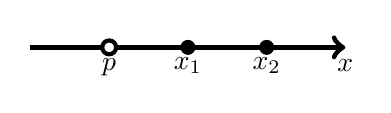
\begin{tikzpicture}[baseline={(0,0.25)}]
\draw [->,line width=2pt](-2,0) -- (2,0) node[below] {$x$};
\draw [fill=white, draw=black, line width=1.5pt] (-1,0) circle (2.5pt) node[below] {$p$};
\draw [fill=black] (0,0) circle (2.5pt) node[below] {$x_1$};
\draw [fill=black] (1,0) circle (2.5pt) node[below] {$x_2$};
\end{tikzpicture}} &
$\left\{\begin{aligned}
&D\greater 0\\
&af(p)\greater 0\\
&p\less x_0
\end{aligned}\right.$\\\hline
\adjustbox{valign=c}{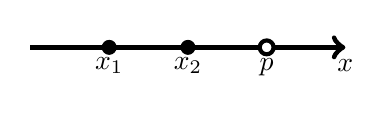
\begin{tikzpicture}[baseline={(0,0.25)}]
\draw [->,line width=2pt](-2,0) -- (2,0) node[below] {$x$};
\draw [fill=black] (-1,0) circle (2.5pt) node[below] {$x_1$};
\draw [fill=black] (0,0) circle (2.5pt) node[below] {$x_2$};
\draw [fill=white, draw=black, line width=1.5pt] (1,0) circle (2.5pt) node[below] {$p$};
\end{tikzpicture}} &
$\left\{\begin{aligned}
&D\greater 0\\
&af(p)\greater 0\\
&x_0\less p
\end{aligned}\right.$\\\hline
\adjustbox{valign=c}{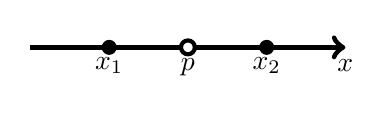
\begin{tikzpicture}[baseline={(0,0.25)}]
\draw [->,line width=2pt](-2,0) -- (2,0) node[below] {$x$};
\draw [fill=black] (-1,0) circle (2.5pt) node[below] {$x_1$};
\draw [fill=white, draw=black, line width=1.5pt] (0,0) circle (2.5pt) node[below] {$p$};
\draw [fill=black] (1,0) circle (2.5pt) node[below] {$x_2$};
\end{tikzpicture}} &
$af(p)\less 0$
\end{sheet*}

\subsection{Метод неопределённых коэффициентов}

{\bold Метод неопределённых коэффициентов} применяется для вычисления коэффициентов выражений, вид которых {\ital заранее известен}.

\begin{theorem}
{\bold Теорема.} Пусть $P(x)$, $G(x)$ --- многочлены одинаковой степени. Они {\ital равны}, если:
% ---
$$p_i=g_i,\ \forall i\in[0;n]$$ 
\end{theorem}

\subsection{Формулы Виета}

\begin{theorem}
{\bold Формулы Виета.} Для многочлена $n$-ой степени и его $n$~корней справедливы соотношения:

{\centering\begin{tblr}{colspec={c@{\qquad}c}}
$\displaystyle x_1+\dots+x_n=-\frac{a_1}{a_0}$ & \SetCell[r=2]{c}$\displaystyle x_1\dots x_n=(-1)^{n}\frac{a_n}{a_0}$\\
$\displaystyle x_1x_2+\dots+x_{n-1}x_n=\frac{a_2}{a_0}$\\
\end{tblr}\par}
\end{theorem}

{\bold Идея.} Разложим многочлен на {\ital линейные множители} с~неизвестными корнями.

После упрощения воспользуемся {\ital методом неопределённых коэффициентов}.

\subsection{Избавление от иррациональности}

\begin{theorem}
{\bold Факт.} Дробь с иррациональностью в знаменателе можно представить в виде {\ital комбинации} иррациональностей:
% ---
$$\begin{aligned}\frac{1}{1+\sqrt{2}+\sqrt{3}}&=A+B\sqrt{2}+C\sqrt{3}+D\sqrt{6}\\
\frac{1}{2-\sqrt[3]{2}}&=A+B\sqrt[3]{2}+C\sqrt[3]{4}
\end{aligned}$$
\end{theorem}
% ---
Этот факт имеет сложное доказательство, которое косвенно есть на сайте МГУ. 
